
\section{Expérimentations}

Dans cette section, nous évaluons l'impact de l'adaptabilité de \SPRAY sur les
métriques communément employées dans l'étude des performances de protocoles
d'échantillonnage de pairs. Ceux-ci incluent le coefficient de clustering, la
taille moyenne du plus petit chemin, la distribution du nombre de connexions
entrantes, le nombre d'arcs, et les composantes connexes. \CYCLON constitue
l'approche à taille fixe avec laquelle nous comparerons les résultats en lien
avec l'adaptabilité. Les résultats attendus sont :
\begin{inparaenum}
\item des propriétés identiques pour les deux approches lorsque \CYCLON est
  configuré de manière optimale,
\item une meilleure efficacité de \SPRAY lorsque les vues partielles de \CYCLON
  sont trop grande par rapport à la taille du réseau,
\item une plus grande robustesse lorsque les vues partielles de \CYCLON sont
  trop petites par rapport à la taille du réseau.
\item Enfin, contrairement à \CYCLON, \SPRAY possède des doublons dans ses vues
  partielles. Toutefois, ce nombre de doublons est supposé négligeable.
\end{inparaenum}
\SCAMP constitue l'approche avec laquelle nous comparerons \SPRAY lorsque nous
examinerons les échecs dans l'établissement des connexions. Nous nous attendons
à ce que \SCAMP échoue à maintenir un réseau connecté, contrairement à \SPRAY.

Les expérimentations ont été exécuté sur le simulateur
\PEERSIM~\cite{montresor2009peersim}. Le code relatif aux protocoles
d'échantillonnages \CYCLON, \SCAMP, et \SPRAY sont disponibles sur la
plate-forme Github\footnote{\url{http://github.com/justayak/peersim-spray}}.

\begin{figure*}
  \centering
  \subfloat[Figure A][Clustering coefficient of \CYCLON.]{
    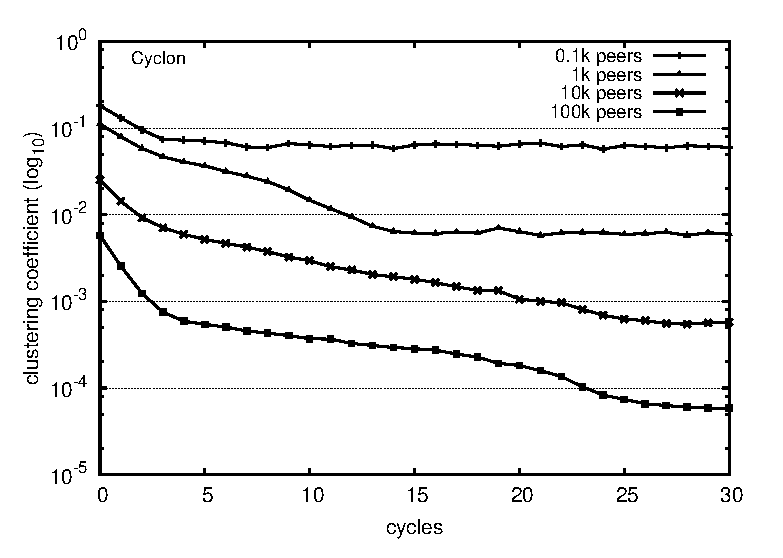
\includegraphics[width=0.47\textwidth]{img/spray/cycloncluster.eps}}
  \hspace{10pt}
  \subfloat[Figure B][Clustering coefficient of \SPRAY.]{
    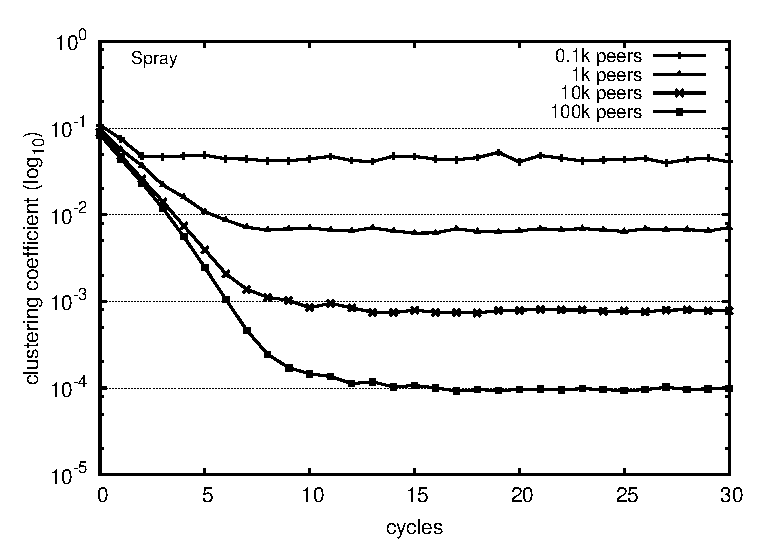
\includegraphics[width=0.47\textwidth]{img/spray/spraycluster.eps}}
  \caption{\label{fig:spray:clustering}The x-axis denotes the elapsed time in
    cycles while the y-axis denotes the $\log_{10}$-scaled clustering
    coefficient.}
\end{figure*}

\begin{asparadesc}
\item [Objectif:] Montrer comment l'adaptabilité influence le clustering et le
  temps de convergence.
\item [Description:] Le coefficient de clustering moyen $\overline{C}$ mesure la
  connexité du voisinage de chaque pair dans le réseau :
  \begin{equation}
    \overline{C} = {1\over |\mathcal{N}|}\sum\limits_{x\in\mathcal{N}}C_x
  \end{equation}
  où $C_x$ est le coefficient de clustering local du pair $p_x$. L'expérience
  implique 0.1k, 1k, 10k, et 100k pairs. Le représentant des approches à taille
  fixe est \CYCLON. Ce dernier est configuré de manière optimale pour 1k pairs
  ($\ln(1000)\approx 7$ voisins). Durant les échanges, les pairs utilisant
  \CYCLON mélangent 3 de leurs 7 voisins. Ainsi, les vues partielles de \CYCLON
  sont trop grandes pour 0.1k pairs, et trop petites pour 10k et 100k pairs.
\item [Résultat:] La figure~\ref{fig:spray:clustering} montre que \CYCLON
  démarre avec un coefficient de clustering plus bas que \SPRAY. Malgré cela,
  \SPRAY parvient à converger plus rapidement que \CYCLON. De plus, quand le
  nombre de pairs augmente dans le réseau, le temps de convergence de \CYCLON en
  souffre fortement. À l'opposé, \SPRAY converge très rapidement quel que soit
  la taille du réseau. La figure~\ref{fig:spray:clustering} montre aussi que les
  deux approches convergent vers un coefficient de clustering bas
  caractéristique des graphes aléatoires. Néanmoins, \CYCLON et \SPRAY
  n'atteignent pas les mêmes valeurs après convergence. À l'exception du cas où
  \CYCLON est configuré de manière optimale, les valeurs obtenus par \SPRAY sont
  soit au dessous (lorsque les vues de \CYCLON sont trop grandes) ou au dessus
  (lorsque les vues de \CYCLON sont trop petites). Globalement, cela montre que
  \SPRAY
  \begin{inparaenum}[(i)]
  \item converge vers un coefficient de clustering stable,
  \item qui reflète les besoins dû à la taille du réseau.
  \end{inparaenum}
  Cela a une influence sur l'équilibrage des charges et la robustesse par
  rapport aux allées et venues de pairs.    
\item [Explications:] \CYCLON commence avec un coefficient de clustering plus
  petit car lorsqu'un pair rejoint le réseau, un cheminement aléatoire est
  effectué afin d'en faire l'annonce. Ainsi, le réseau de départ est déjà
  légèrement équilibré au moment où la simulation commence les échanges de vue
  partielle. À l'opposé, un nouvel arrivant avec \SPRAY n'annonce son entrée
  qu'au voisinage de son contact. De ce fait, le réseau est fortement
  déséquilibré au départ de l'expérience, quelle que soit taille du
  réseau. Malgré cela, \CYCLON ne converge pas aussi vite que \SPRAY vers un
  coefficient stable. Cela est due à la taille fixe de sa vue partielle qui
  contraint la qualité des échanges. Le coefficient de clustering mesure la
  connexité du voisinage de chaque pair dans le réseau. Cela dépend donc de la
  taille de vue partielle qui, pour \CYCLON, est fixé lors de la configuration.
  Ainsi lorsque le nombre de pairs est multiplié par 10, le coefficient de
  clustering est divisé par 10. En revanche, les pairs utilisant \SPRAY ont une
  taille de vue partielle pouvant varier afin de refléter la taille du réseau.
  Ainsi, quand le réseau contient 1k pairs, les vues partielles s'adaptent à
  cette taille. Par conséquent, \SPRAY est très légèrement en dessous de \CYCLON
  dans ce scénario car la taille moyenne de vue partielle est de 7.4 pour ce
  premier contre 7 pour ce second. En étendant ce raisonnement aux autres
  tailles de réseau, cela explique pourquoi \SPRAY converge vers une valeur plus
  basse lorsque les vues partielles de \CYCLON sont trop grandes, et vers une
  valeur plus haute lorsque les vues partielles de \CYCLON sont trop petites.
\end{asparadesc}

\begin{figure}
  \centering
  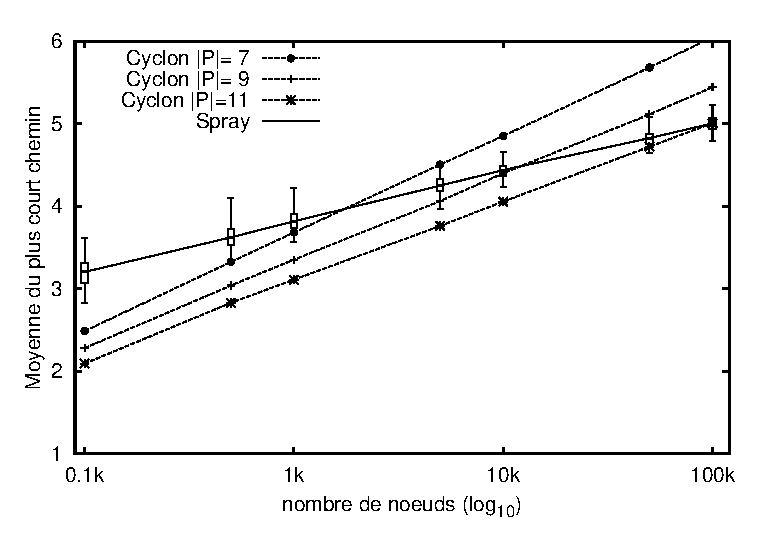
\includegraphics[width=.8\textwidth]{img/spray/avgpath.eps}
  \caption{\label{fig:avgpath}The average shortest path length of \SPRAY and
    \CYCLON. The x-axis denotes the number of peers in the network on a
    $\log_{10}$ scale (from 100 to 100k peers) while the y-axis denotes the
    average shortest path length of the network.}
\end{figure}

\begin{figure}
  \centering
  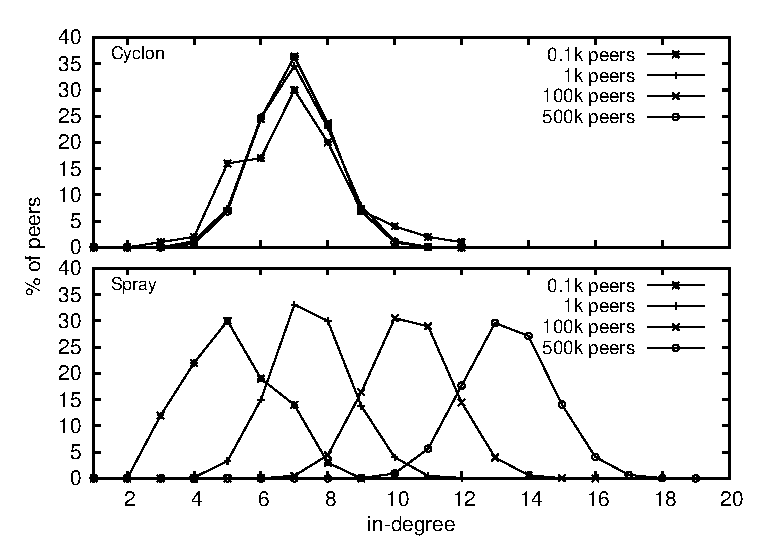
\includegraphics[width=.8\textwidth]{img/spray/histo.eps}
  \caption{\label{fig:histo}The in-degree distribution of \CYCLON and
    \SPRAY. The x-axis denotes the in-degree in number of nodes while the
    y-axis indicates the percentage of peers with such in-degree. The top
    figure is dedicated to the runs concerning \CYCLON while the bottom figure
    concerns \SPRAY.}
\end{figure}

\begin{figure*}
  \centering
  \subfloat[Figure A][\label{fig:churnA}The x-axis denotes the
  elapsed time in cycles. The upper graph y-axis shows the number of total
  connections in the overlay while the lower graph y-axis shows the variance
  $\sigma^2$ of the partial view sizes in the network.]{
    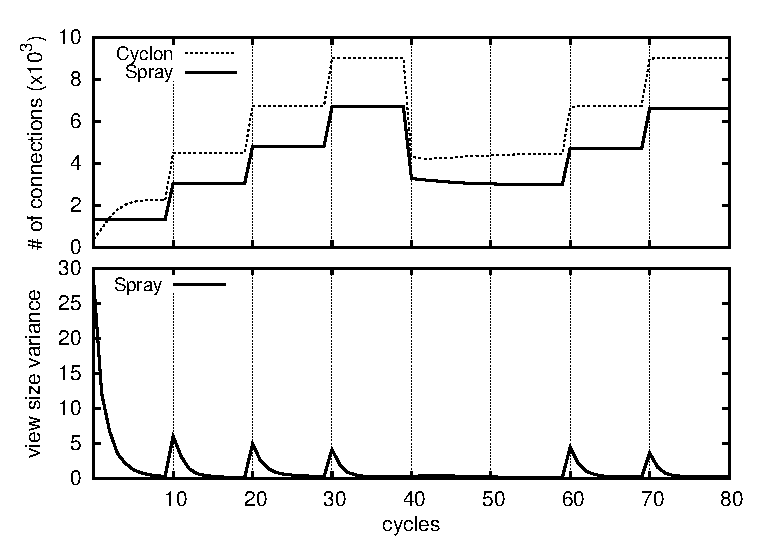
\includegraphics[width=0.47\textwidth]{img/spray/churn.eps}}
  \hspace{10pt}
  \subfloat[Figure B][\label{fig:churnB}The x-axis denotes the
  elapsed time in cycles. The y-axis denotes the average partial view size.]{
    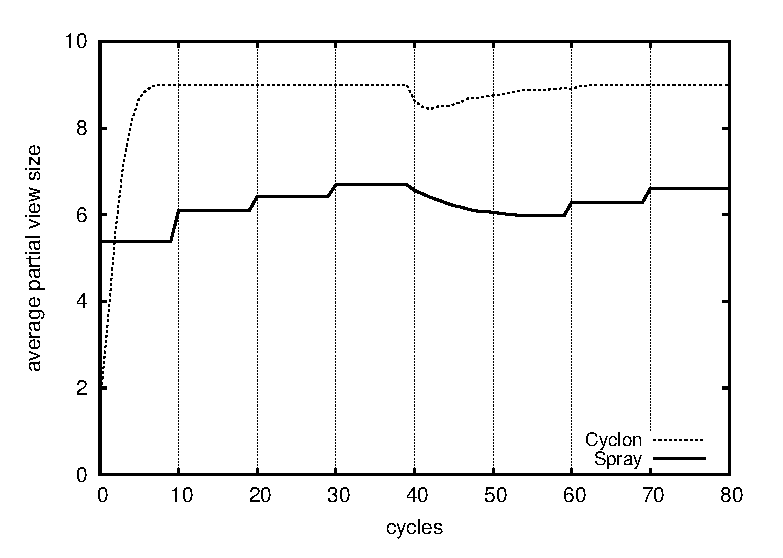
\includegraphics[width=0.47\textwidth]{img/spray/avgpv.eps}}
  \caption{\label{fig:churn}\CYCLON (partial view size configured to 9) and
    \SPRAY in a dynamic network. 2.5k peers join the network at cycles $0$,
    $10$, $20$, and $30$. Then 5k peers leave at cycle $40$. Finally 2.5k peers
    join at cycles $60$ and $70$. The final network contains 10k members.}
\end{figure*}

\begin{figure}
  \centering
  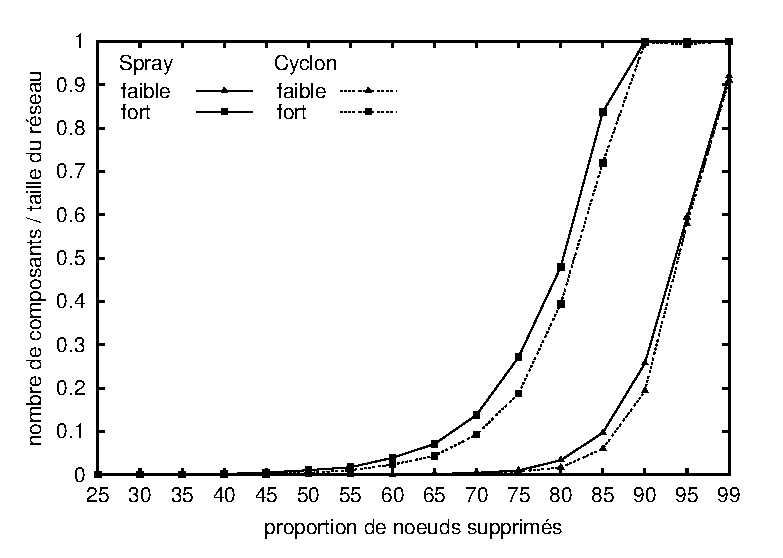
\includegraphics[width=.8\textwidth]{img/spray/resilience.eps}
  \caption{\label{fig:resilience}Robustness of \CYCLON and \SPRAY to massive
    failures. The x-axis denotes the percentage of peers removed at once in a
    network containing 10k members. The y-axis denotes the number of
    components over the current network size (after the removals). The
    measurements concern the weak and strong components which basically means
    the number clusters in undirected or directed graph respectively.}
\end{figure}


\begin{figure}
  \centering
  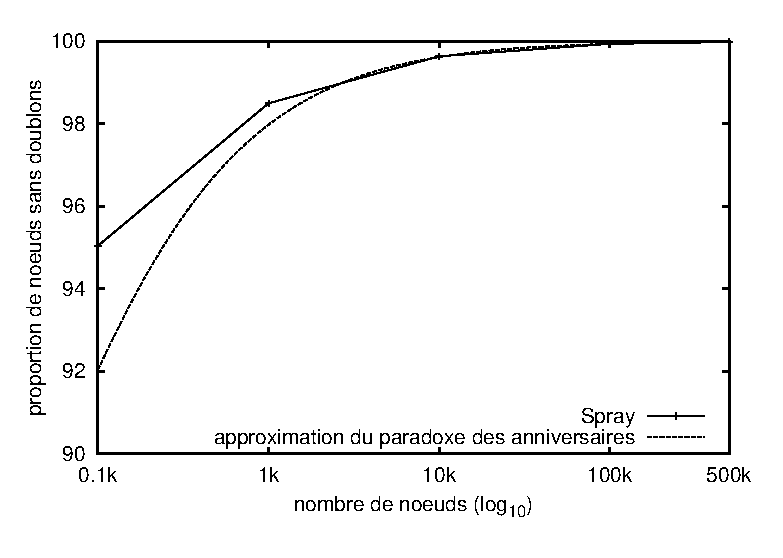
\includegraphics[width=.8\textwidth]{img/spray/duplicates.eps}
  \caption{\label{fig:duplicates}Duplicates in networks of different size: the
    $\log_{10}$-scaled x-axis denotes the network size while y-axis denotes the
    proportion of peers without any duplicates in their partial view.}
\end{figure}

\begin{figure}
  \centering 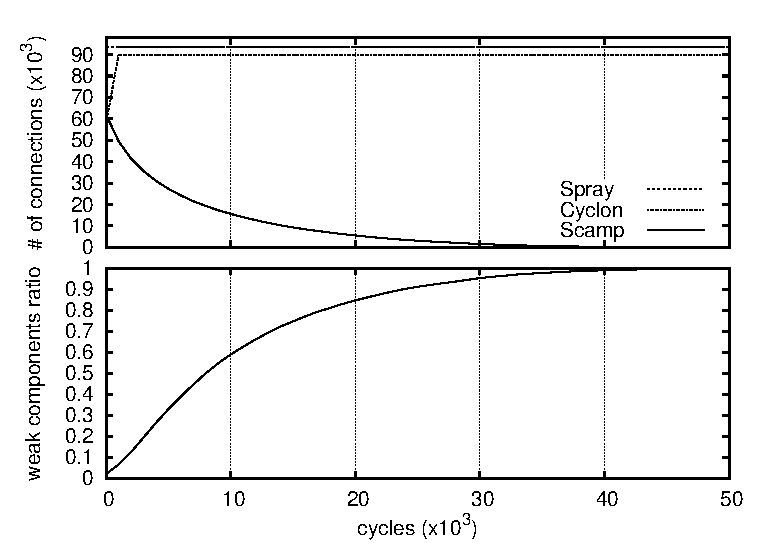
\includegraphics[width=.8\textwidth]{img/spray/degen.eps}
  \caption{\label{fig:degeneration}\CYCLON, \SCAMP, and \SPRAY in network
    subject to failures in the connection establishments. The x-axis denotes
    the elapsed time in cycles ($10^3$-scaled). The y-axis of the top figure
    denotes the global number of arcs ($10^3$-scaled). The y-axis of the bottom
    figure denotes the ratio of weak components over the current network size.}
\end{figure}

%%% Local Variables:
%%% mode: latex
%%% TeX-master: "../../paper"
%%% End:
